\documentclass[border=6pt]{standalone}
% Shared preamble for figures.  Each figure is a standalone .tex in
% figures/Unit_X/ that \input's this file; scripts/make-figures.sh turns it
% into images/Unit_X/<name>.svg.  The lesson page and the guided notes both
% use that one SVG, so a figure is drawn once.
%
% Key figures: a figure whose .tex uses \ifkey ... \fi also gets a
% <name>_KEY.svg, built with \keytrue.  Draw the answers inside \ifkey, in
% the key colour (\ans{} for a label, the "answer" style for lines).
\usepackage[T1]{fontenc}
\usepackage{helvet}
\renewcommand{\familydefault}{\sfdefault}
\usepackage{amsmath}
\usepackage{tikz}
\usetikzlibrary{arrows.meta,calc,angles,quotes,decorations.markings,decorations.pathreplacing}
% axis numbers in the text font, not math italic
\pgfkeys{/pgf/number format/.cd,assume math mode=true,1000 sep={}}

\newif\ifkey
\ifdefined\iskey\keytrue\fi
\definecolor{key}{HTML}{C0192B}      % same red as the guided-notes keys
\newcommand{\ans}[1]{\textcolor{key}{\bfseries #1}}

\tikzset{
  % points: \fill (A) circle[radius=\ptr];
  every picture/.append style={line cap=round, line join=round, >={Stealth[length=2.6mm,width=2mm]}},
  fig/.style={thick},
  line/.style={thick,<->},            % a line goes on forever both ways
  ray/.style={thick,->},              % a ray goes on forever one way
  answer/.style={very thick,key},
  % congruence ticks at the middle of a segment: \draw[tick1] (A) -- (B);
  tick1/.style={postaction={decorate},decoration={markings,
    mark=at position .5 with {\draw[thick] (0,-2.2pt) -- (0,2.2pt);}}},
  tick2/.style={postaction={decorate},decoration={markings,
    mark=at position .5 with {\draw[thick] (-1.3pt,-2.2pt) -- (-1.3pt,2.2pt) (1.3pt,-2.2pt) -- (1.3pt,2.2pt);}}},
  tick3/.style={postaction={decorate},decoration={markings,
    mark=at position .5 with {\draw[thick] (-2.4pt,-2.2pt) -- (-2.4pt,2.2pt) (0,-2.2pt) -- (0,2.2pt) (2.4pt,-2.2pt) -- (2.4pt,2.2pt);}}},
  % parallel arrows at the middle of a line: \draw[par1] (A) -- (B);
  par1/.style={postaction={decorate},decoration={markings,
    mark=at position .5 with {\draw[thick] (-2.5pt,-2.5pt) -- (0,0) -- (-2.5pt,2.5pt);}}},
  par2/.style={postaction={decorate},decoration={markings,
    mark=at position .5 with {\draw[thick] (-4pt,-2.5pt) -- (-1.5pt,0) -- (-4pt,2.5pt) (-1pt,-2.5pt) -- (1.5pt,0) -- (-1pt,2.5pt);}}},
  % angle arcs: \pic[ang] {angle = A--B--C};  ang2 for a second matching angle
  ang/.style={draw,thick,angle radius=5mm},
  ang2/.style={draw,thick,angle radius=5mm,double,double distance=1.2pt},
  % right-angle box: \pic[rt] {right angle = A--B--C};
  rt/.style={draw,thick,angle radius=2.6mm},
}
\newcommand{\ptr}{2pt}
% a labelled point: \pt{A}{(x,y)}{above left}
\newcommand{\pt}[3]{\coordinate (#1) at #2; \fill (#1) circle[radius=\ptr] node[#3] {$#1$};}

% coordinate plane with every unit gridded: \cgrid{xmin}{xmax}{ymin}{ymax}{label step}
% Grid lines every unit. Tick labels every <label step> units, but never closer
% than about 0.55cm: on a small grid a step of 1 becomes 2 (or 5), so the
% numbers do not run into each other. Labels sit on white so grid lines
% do not cross them.
% To leave out tick labels where a curve crosses an axis, before \cgrid:
%   \renewcommand{\cgskipx}{5,-5}  \renewcommand{\cgskipy}{5}
\newcommand{\cgskipx}{}\newcommand{\cgskipy}{}
\makeatletter
\newcommand{\cgrid}[5]{%
  \pgfpointxy{1}{0}\pgfmathsetmacro{\cgunit}{\pgf@x}%
  \pgfmathtruncatemacro{\cgs}{max(#5, (\cgunit*#5 < 15.6) ? 2 : #5, (\cgunit*#5 < 7.9) ? 5 : #5)}%
  \draw[gray!45,thin,step=1] (#1,#3) grid (#2,#4);  % step=1 is one unit; the default is 1cm
  % axes run at least 0.5cm past the last grid line, so the arrowheads clear
  % the end tick labels on a small grid
  \pgfmathsetmacro{\cgo}{max(0.4, 14.2/\cgunit)}%
  \draw[thick,<->] (#1-\cgo,0) -- (#2+\cgo,0) node[right] {$x$};
  \draw[thick,<->] (0,#3-\cgo) -- (0,#4+\cgo) node[above] {$y$};
  \pgfmathtruncatemacro{\cgxa}{ceil((#1)/\cgs)*\cgs}\pgfmathtruncatemacro{\cgxb}{\cgxa+\cgs}%
  \pgfmathtruncatemacro{\cgya}{ceil((#3)/\cgs)*\cgs}\pgfmathtruncatemacro{\cgyb}{\cgya+\cgs}%
  \foreach \t in {\cgxa,\cgxb,...,#2} {\edef\cgt{,\t,}\expandafter\in@\expandafter{\cgt}{,\cgskipx,}\ifin@\else\ifnum\t=0\else\node[below,font=\scriptsize,fill=white,inner sep=1pt,yshift=-1pt] at (\t,0) {\t};\fi\fi}
  \foreach \t in {\cgya,\cgyb,...,#4} {\edef\cgt{,\t,}\expandafter\in@\expandafter{\cgt}{,\cgskipy,}\ifin@\else\ifnum\t=0\else\node[left,font=\scriptsize,fill=white,inner sep=1pt,xshift=-1pt] at (0,\t) {\t};\fi\fi}}
\makeatother

\begin{document}
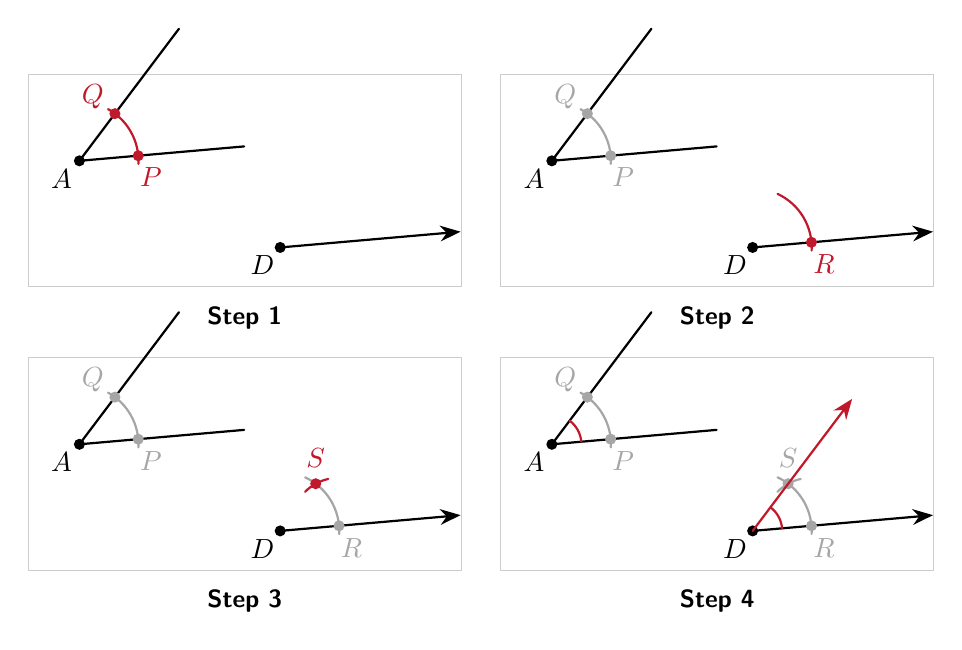
\begin{tikzpicture}[x=1cm,y=1cm]
\path (0,0) rectangle (5.5,2.7);
\draw[gray!40,thin] (0,0) rectangle (5.5,2.7);
\draw[fig] (0.65,1.6) -- (2.742,1.783);
\draw[fig] (0.65,1.6) -- (1.914,3.277);
\fill[black] (0.65,1.6) circle[radius=\ptr]; \node[] at (0.424,1.374) {$A$};
\draw[fig,->] (3.2,0.5) -- (5.491,0.7);
\fill[black] (3.2,0.5) circle[radius=\ptr]; \node[] at (2.974,0.274) {$D$};
\draw[key,thick] (1.399,1.561) arc[start angle=-3,end angle=61,radius=0.75];
\fill[key] (1.397,1.665) circle[radius=\ptr]; \node[text=key] at (1.557,1.388) {$P$};
\fill[key] (1.101,2.199) circle[radius=\ptr]; \node[text=key] at (0.821,2.419) {$Q$};
\node[font=\small\bfseries] at (2.75,-0.4) {Step 1};
\path (6,0) rectangle (11.5,2.7);
\draw[gray!40,thin] (6,0) rectangle (11.5,2.7);
\draw[fig] (6.65,1.6) -- (8.742,1.783);
\draw[fig] (6.65,1.6) -- (7.914,3.277);
\fill[black] (6.65,1.6) circle[radius=\ptr]; \node[] at (6.424,1.374) {$A$};
\draw[fig,->] (9.2,0.5) -- (11.491,0.7);
\fill[black] (9.2,0.5) circle[radius=\ptr]; \node[] at (8.974,0.274) {$D$};
\draw[gray!70,thick] (7.399,1.561) arc[start angle=-3,end angle=61,radius=0.75];
\fill[gray!70] (7.397,1.665) circle[radius=\ptr]; \node[text=gray!70] at (7.557,1.388) {$P$};
\fill[gray!70] (7.101,2.199) circle[radius=\ptr]; \node[text=gray!70] at (6.821,2.419) {$Q$};
\draw[key,thick] (9.949,0.461) arc[start angle=-3,end angle=65,radius=0.75];
\fill[key] (9.947,0.565) circle[radius=\ptr]; \node[text=key] at (10.107,0.288) {$R$};
\node[font=\small\bfseries] at (8.75,-0.4) {Step 2};
\path (0,-3.6) rectangle (5.5,-0.9);
\draw[gray!40,thin] (0,-3.6) rectangle (5.5,-0.9);
\draw[fig] (0.65,-2) -- (2.742,-1.817);
\draw[fig] (0.65,-2) -- (1.914,-0.323);
\fill[black] (0.65,-2) circle[radius=\ptr]; \node[] at (0.424,-2.226) {$A$};
\draw[fig,->] (3.2,-3.1) -- (5.491,-2.9);
\fill[black] (3.2,-3.1) circle[radius=\ptr]; \node[] at (2.974,-3.326) {$D$};
\draw[gray!70,thick] (1.399,-2.039) arc[start angle=-3,end angle=61,radius=0.75];
\fill[gray!70] (1.397,-1.935) circle[radius=\ptr]; \node[text=gray!70] at (1.557,-2.212) {$P$};
\fill[gray!70] (1.101,-1.401) circle[radius=\ptr]; \node[text=gray!70] at (0.821,-1.181) {$Q$};
\draw[gray!70,thick] (3.949,-3.139) arc[start angle=-3,end angle=65,radius=0.75];
\fill[gray!70] (3.947,-3.035) circle[radius=\ptr]; \node[text=gray!70] at (4.107,-3.312) {$R$};
\draw[key,thick] (3.81,-2.44) arc[start angle=103,end angle=135,radius=0.61];
\fill[key] (3.651,-2.501) circle[radius=\ptr]; \node[text=key] at (3.651,-2.181) {$S$};
\node[font=\small\bfseries] at (2.75,-4) {Step 3};
\path (6,-3.6) rectangle (11.5,-0.9);
\draw[gray!40,thin] (6,-3.6) rectangle (11.5,-0.9);
\draw[fig] (6.65,-2) -- (8.742,-1.817);
\draw[fig] (6.65,-2) -- (7.914,-0.323);
\fill[black] (6.65,-2) circle[radius=\ptr]; \node[] at (6.424,-2.226) {$A$};
\draw[fig,->] (9.2,-3.1) -- (11.491,-2.9);
\fill[black] (9.2,-3.1) circle[radius=\ptr]; \node[] at (8.974,-3.326) {$D$};
\draw[gray!70,thick] (7.399,-2.039) arc[start angle=-3,end angle=61,radius=0.75];
\fill[gray!70] (7.397,-1.935) circle[radius=\ptr]; \node[text=gray!70] at (7.557,-2.212) {$P$};
\fill[gray!70] (7.101,-1.401) circle[radius=\ptr]; \node[text=gray!70] at (6.821,-1.181) {$Q$};
\draw[gray!70,thick] (9.949,-3.139) arc[start angle=-3,end angle=65,radius=0.75];
\fill[gray!70] (9.947,-3.035) circle[radius=\ptr]; \node[text=gray!70] at (10.107,-3.312) {$R$};
\draw[gray!70,thick] (9.81,-2.44) arc[start angle=103,end angle=135,radius=0.61];
\fill[gray!70] (9.651,-2.501) circle[radius=\ptr]; \node[text=gray!70] at (9.651,-2.181) {$S$};
\draw[key,thick,->] (9.2,-3.1) -- (10.464,-1.423);
\draw[key,thick] (7.024,-1.967) arc[start angle=5,end angle=53,radius=0.375];
\draw[key,thick] (9.574,-3.067) arc[start angle=5,end angle=53,radius=0.375];
\node[font=\small\bfseries] at (8.75,-4) {Step 4};
\end{tikzpicture}
\end{document}
